\section{Experimentos y Resultados}
% Para la experimentación realizada en este trabajo decidimos comenzar implementando la estrategia \textbf{Grid search},
% la cual nos permitio encontrar la mejor configuracion de hiperparametros entre un subconjunto creado por nosotros. Estos
% hiperparametros son: \textit{learning rate} y \textit{discount} para el algoritmo de \textbf{QLearning}, y el epsilon para
% la politica de control \textbf{$\epsilon-greedy$}. La busqueda fue realizada entre los siguientes valores de cada uno:
%
% \begin{itemize}
%   \item  \textbf{$\epsilon$} = 0.1, 0,2
%   \item \textbf{learning\_rate} = 0.1, 0.2, 0.4, 0.6, 0.8, 0.9, 1.0
%   \item \textbf{discount} = 0.5, 0.6, 0.7, 0.8, 0.9
% \end{itemize}
%
%
% Obteniendo como mejor resultado la siguiente configuracion:
%
% \begin{itemize}
%   \item  \textbf{$\epsilon$} = 0.1
%   \item \textbf{learning\_rate} = 0.4
%   \item \textbf{discount} = 0.9
% \end{itemize}
%
% Ademas de estos hiperparametros para el algoritmo y la politica elegida, tambien necesitamos una cantidad de epocas para
% entrenar y un oponente contra quien jugar.
% Así que tomamos algunas decisiones:

Para la experimentación realizada utilizamos el algoritmo de \textbf{QLearning} para entrenar al agente que jugara al 4 en linea. Este algoritmo utiliza los hiperparametros \textit{learning rate} y \textit{discount} y los valores de inicialización
 de la matriz de valores de Q. Ademas de estos hiperparametros, necesitamos una politica de control, una cantidad de epocas para entrenar y un oponente contra quien jugar.  \\

Tratar todas las combinaciones posibles de parametros no es posible computacionalmente, por este motivo tomamos algunas decisiones sobre los parametros a utilizar, que se irán modificando en función de lo aprendido en el camino:

\begin{enumerate}
\item La cantidad de epocas para entrenar serán 200.000
\item La política de control que utilizaremos será \textbf{$\epsilon-greedy$}. Y tendremos que elegir el mejor $\epsilon$
\item Nuestro oponente será random.
\item Utilizaremos gridSearch para setear los valores de \textit{learning rate},  \textit{discount} y el valor con que inicializamos la matriz de Q. Estos tres parametros se moverán entre 0 y 1. Aumentado el valor con pasos de 0.1
\end{enumerate}

Estas deciones achicaron el espacio de exploración pero aun asi era muy grande. Asi que fijamos dos conjuntos de pruebas distintos. 

\begin{itemize}
  \item El primer conjunto lo obtuvimos seteando \textbf{$\epsilon$} en 0.1 y 0.2 para tener un poco de exploración, sin que sea excesiva, \textit{learning rate} a 0.4, 0.5 y 0.6 para que aprenda más o menos equlibrado de la experiencia reciente y la pasada y \textit{discount} en 0.8, 0.9 y 1.0 para darle mayor importancia a las recompensas futuras. Por ultimo los valores iniciales de la matriz de Q los seteamos en 0, 1 y valores random. 
   
  \item  El segundo conjunto lo armamos haciendo varias corridas en las que en cada una movimos un unico parametro y dejamos fijo al resto. Cada vez que obtuvimos el mejor paramtro de la iteracion lo fijamos y movimos el siguiente. Cada uno de los paramtros fué movido entre 0 y 1 con pasos de 0.1. La combinación inicial fué la matriz de Q en 0 y en valores random, el \textit{learning rate} y \textit{discount} a 0.5, con el objetivo de tomar por igual las recompensas futuras y las actuales, de igual forma con la información reciente y la pasada. \\
\end{itemize} 

El armado de estos dos conjuntos de parametros nos redujo considerablemente la cantidad de combinaciones a probar y el tiempo de computo. Sin embargo seguia siendo muy alto, motivo por el cual se nos ocurrió que en vez de jugar con un tablero de 7x6 y 4 en linea, podíamos acotarlo a un 3 en linea con un tablero de 6x5. Con la hipotesis de que si lograbamos tener un buen entrenamiento en un tablero mas chico y jugar 3 en linea podemos conseguir con los mismos parametros un buen entrenamiento para el juego 4 en linea.


%La primer combinacion de parametros tardó aproximadamente 10 min en entrenar. Haciendo una proyeccion de cuanto podria tardar en total con todas las combinaciones tardaria aproximadamente 101 dias, otra señal de que teniamos que reducir la cantidad de combinaciones.

\subsection{Experimento 3 en linea en tablero de $6\times5$}

Para el set 1 obtuvimos que el jugador Qlearning ganaba el 89\% de las veces, mientras que para el set 2 ganaba el 93\% con los siguientes conjuntos de paramtros. 

\begin{center}
    \begin{tabular}{| l | l | l |}
    \hline
     					    &  \textbf{Set 1} & \textbf{Set 2} \\ \hline
    \textbf{$\epsilon$}     &  0.1   		  & 0.0   \\
    \textbf{learning\_rate} &  0.4   		  & 0.9   \\ 
    \textbf{discount}       &  0.9  		  & 0.5   \\ 
	\textbf{initialQ} 		&  0.0   		  & 0.0   \\
    \hline
    \end{tabular}
\end{center}

Lo que observamos es:
\begin{itemize}
\item El set 1 le da importancia a la exploración mientras que el set 2 no la utiliza. \\
\item El set 1 usa poco la información reciente y el set 2 la utiliza mucho. \\
\item El set 1 le da mucha importancia a las recompensas futuras mientras que el set 2 le da la misma importancia a ambas. \\
\item En ambos casos es mejor aprender los valores de Q a travez del juego evitando tener una estrategia voraz.\\
\end{itemize}

 
Lo que nos llama la atención del Set 2 es que no utiliza exploración. Una vez que encuentra un camino lo utiliza. Asi que decidimos probar la combinación de los mejores parametros para ambos sets agregando valores de epsilon = $[$0.0, 0.0001, 0.001, 0.1$]$

Se obtuvo el 95\% de los juegos ganados para los siguientes parametros:
\begin{center}
    \begin{tabular}{| l | l | l |}
    \hline
     					    &  \textbf{Set 3} \\ \hline
    \textbf{$\epsilon$}     &  0.0001  		  \\
    \textbf{learning\_rate} &  0.4   		  \\ 
    \textbf{discount}       &  0.9  		  \\ 
	\textbf{initialQ} 		&  0.0   		  \\
    \hline
    \end{tabular}
\end{center}


A continuación podemos ver para los diferentes sets los porcetajes de victorias en función de la cantidad de iteraciones:


\begin{figure}[h]
 \centering
 \begin{minipage}{.45\textwidth}
  %\begin{minipage}[c]{1\textwidth}
	\centering
	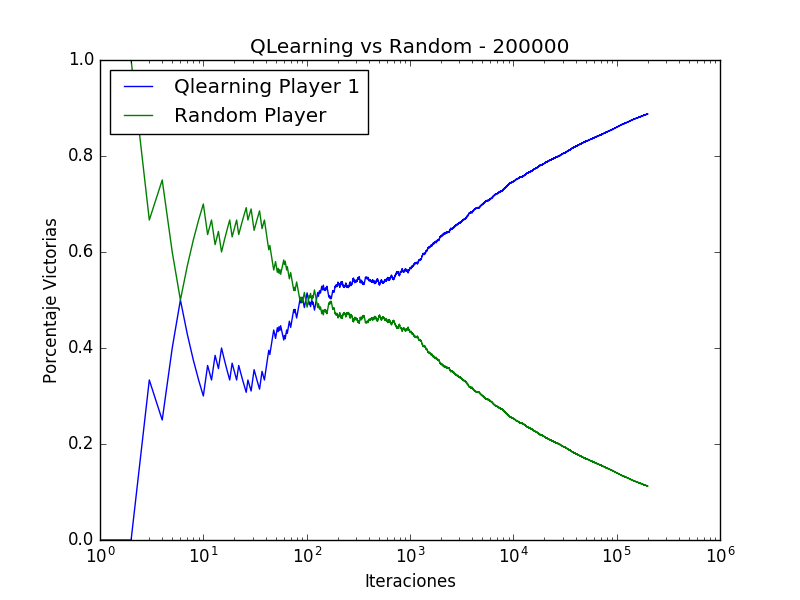
\includegraphics[scale=0.35]{img1/QlearningVsRandom_200000_6x5_hernan.png}
        \caption{Qlearning vs Random 200000 juegos - Set 1}
  \end{minipage}
 \begin{minipage}{.5\textwidth}
	\centering
	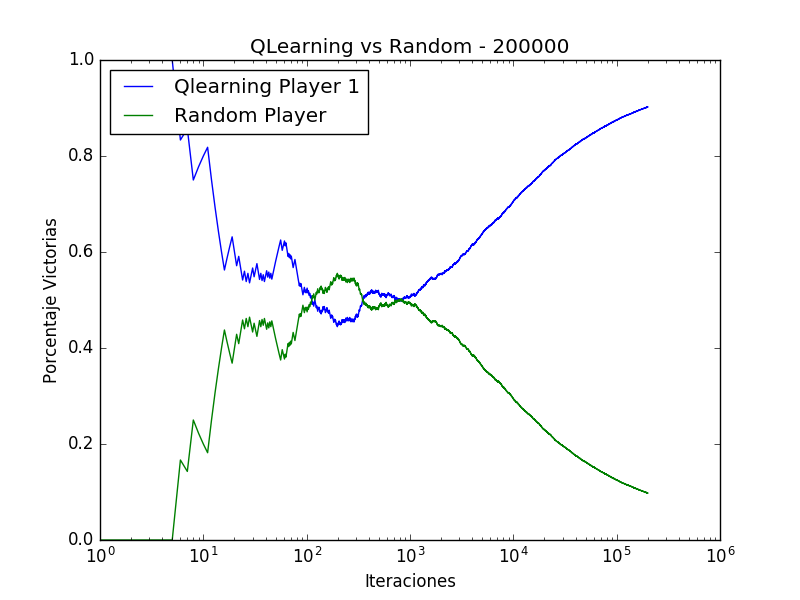
\includegraphics[scale=0.35]{img1/QlearningVsRandom_200000_6x5_cyntia.png}
        \caption{Qlearning vs Random 200000 juegos - Set 2}
  \end{minipage}
\end{figure}


\begin{figure}[h]
 \centering
 \begin{minipage}{.45\textwidth}
  %\begin{minipage}[c]{1\textwidth}
	\centering
	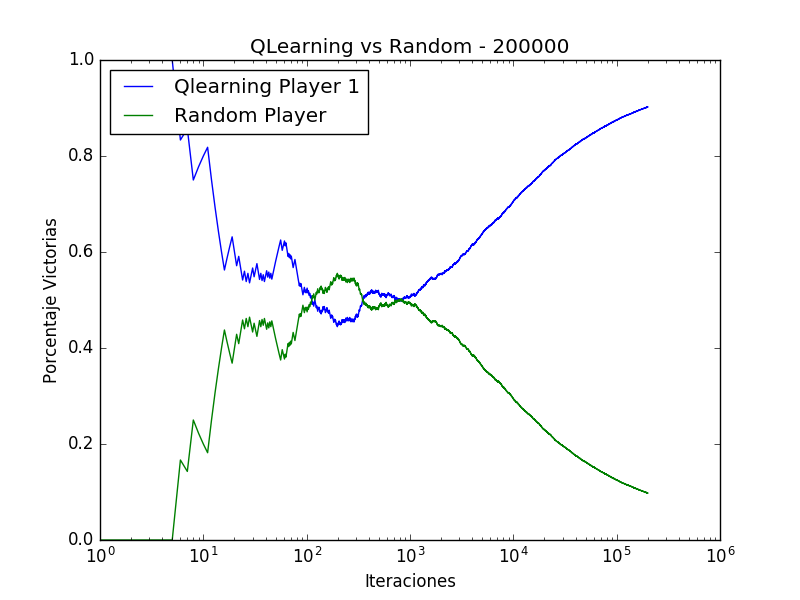
\includegraphics[scale=0.35]{img1/QlearningVsRandom_200000_6x5_cyntia.png}
        \caption{Qlearning vs Random 200000 juegos - Set 3}
  \end{minipage}
\end{figure}

 
%\begin{frame}
%\begin{figure}[h]
% \centering
%  \begin{minipage}[c]{1\textwidth}
%	\centering
%	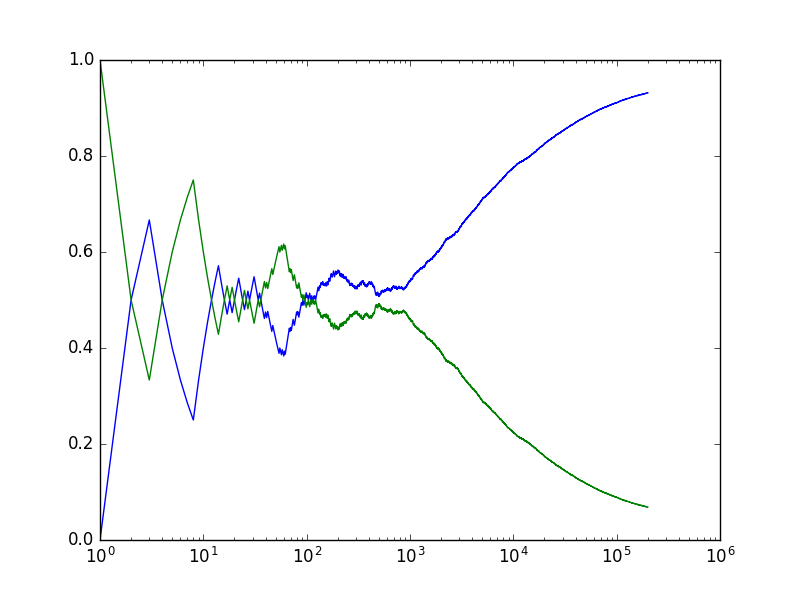
\includegraphics[scale=0.5]{img/QlearningRandomEgreedy200000.png}
%        \caption{Qlearning vs Random 200000 juegos}
%  \end{minipage}
%\end{figure}
%\end{frame}

Lo que podemos observar es que efectivamente el jugador QLearning aprende, pues a medida que aumenta la cantidad de juegos gana mayor cantidad de partidas. Contrariamente al jugador random.  \\

En los tres casos alrededor del orden de $10^{3}$ empieza a ganar el jugador entrenado. Pero considerando que el oponente es random decidimos jugar nosotros para ver cuan bueno era. Lo que notamos luego de varias partidas es que lo que había aprendido era una estrategia ganadora cuando el que ponía la primer ficha era él. Tambi\'en se defend\'ia bien cuando era su turno, es decir, no aprendi\'o algo en detrimento de lo otro.\\

La estregia es muy parecida a la de que se utiliza en el juego de ta-te-ti de formar una L, hace una serie de movimientos que lleva a que el contrincante sin importar donde ponga la pr\'oxima ficha, el Qlearner tiene otras dos posibilidades para ganar. Para que el lector pueda probar esto y jugar, se puede cargar el modelo desde la l\'inea de comando.

Nos pareci\'o muy llamativa este comportamiento que logr\'o el Qlearner, y lo tomamos como una prueba fehaciente que el modelo realmente est\'a aprendiendo la naturaleza detr\'as del juego. Mientras que una persona tardar\'ia bastante tiempo en encontrar la estrategia ganadora, el algoritmo lo encontr\'o simplemente al jugar repetidas veces contra un jugador que tira acciones random.

Y esto explicaría por que no empatan. Como el jugador que comienza tiene una estrategia ganadora siempre va a ganar.\\

Todavía nos llama la atención el valor bajo que usa de exploración. El resto de los parametros nos parecieron bastante razonables en cuanto a balanceo de utilización de recompensas futuras y actuales, información reciente y futura e inicialización de Q.
Para las siguientes pruebas utilzamos el set 3.\\

Nos preguntamos que pasaría si poníamos a jugar a dos Qlearners. Lo que esperabamos ver es lo mismo que pasó cuando se juega contra un jugador random, es decir, en algun momento se encuentra la estrategia ganadora y ganará la partida el que la comienza.\\

A continuación mostramos los resultados de dos jugadores Qlearner para diferente número de iteraciones:

\begin{figure}[h]
 \centering
 \begin{minipage}{.45\textwidth}
  %\begin{minipage}[c]{1\textwidth}
	\centering
	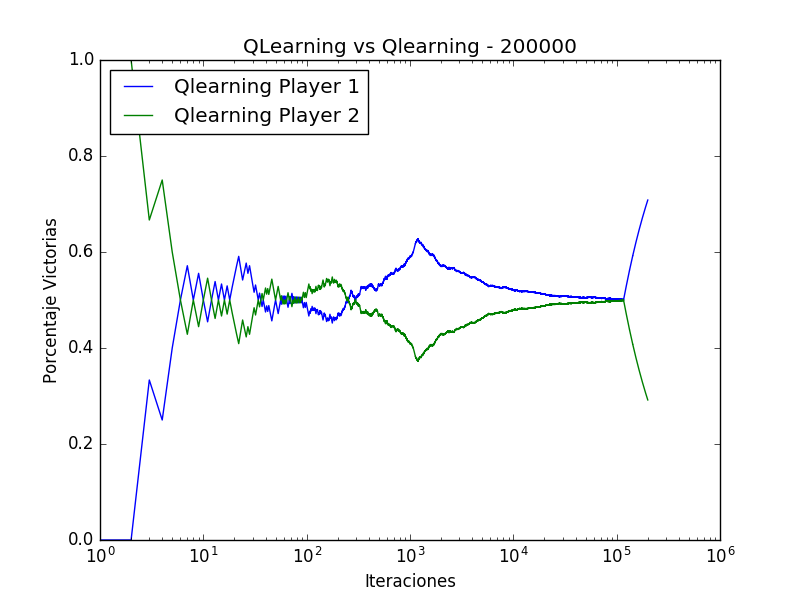
\includegraphics[scale=0.35]{img1/QlearningVsQlearning_200000_6x5_merge.png}
        \caption{Qlearning vs Qlearning 200000 juegos}
  \end{minipage}
 \begin{minipage}{.5\textwidth}
	\centering
	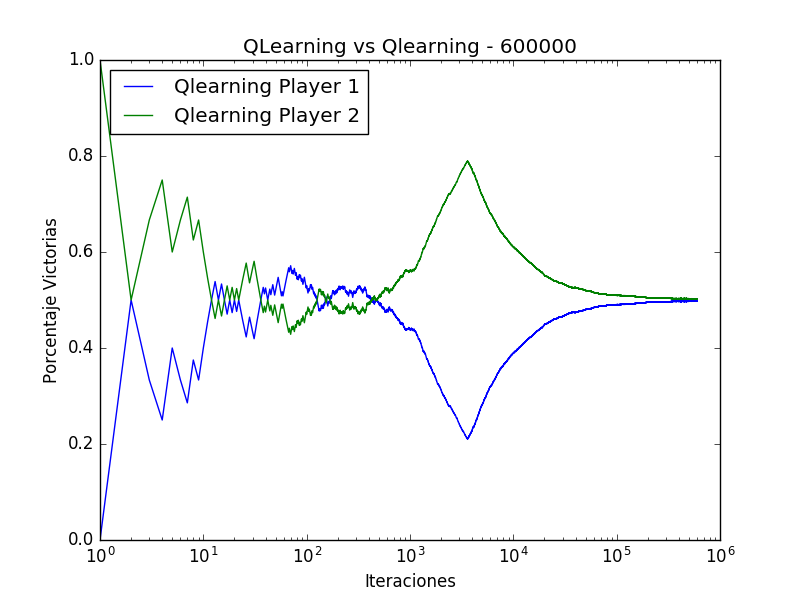
\includegraphics[scale=0.35]{img1/QlearningVsQlearning_600000_6x5_merge.png}
        \caption{Qlearning vs Qlearning 1000000 juegos}
  \end{minipage}
\end{figure}


\begin{figure}[h]
 \centering
 \begin{minipage}{.45\textwidth}
  %\begin{minipage}[c]{1\textwidth}
	\centering
	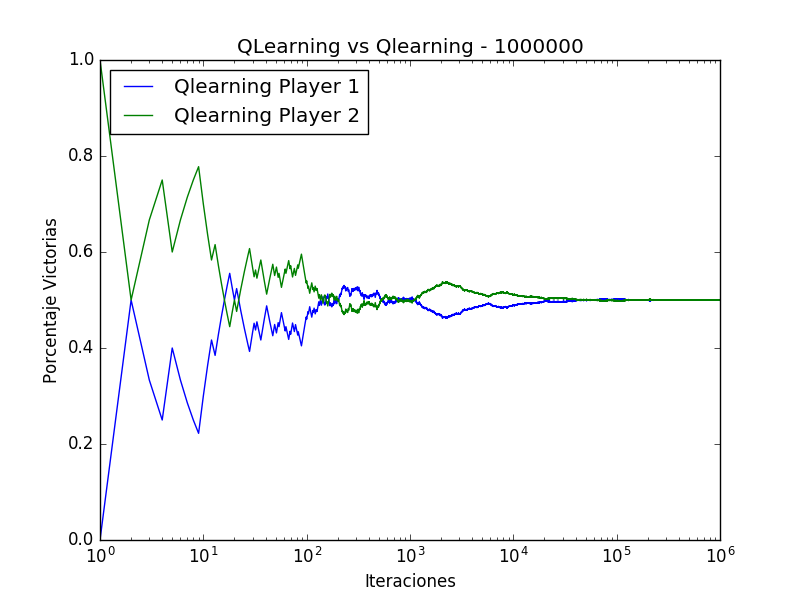
\includegraphics[scale=0.35]{img1/QlearningVsQlearning_1000000_6x5_merge.png}
        \caption{Qlearning vs Qlearning 1000000 juegos}
  \end{minipage}
\end{figure}

Viendo los gráficos creímos que pasaba lo mismo que en el caso anterior. Al aprender una estrategia ganadora en algún momento ganaba siempre el jugador que comenzaba la partida. 

Sin embargo quisimos ver que tan bien había aprendido y nos encontramos con que no aprendió una estrategia ganadora. Creemos que esto tiene que ver con que tener un oponente random hace que se exploren más opciones y por eso, si se utiliza un epsilon ``grande'' se convierte en ``demasiado'' random, pero si se tiene un oponente Qlearner tener un epsilon ``bajo'' lo convierte en ``poco'' random. \\

Entonces nos prenguntamos que pasaría si entrenamos con dos jugadores Qlearners los mismos parametros que usamos anteriormente pero aumentando el epsilon. 

Y obtuvimos lo siguiente:

\begin{figure}[h]
 \centering
 \begin{minipage}{.45\textwidth}
  %\begin{minipage}[c]{1\textwidth}
	\centering
	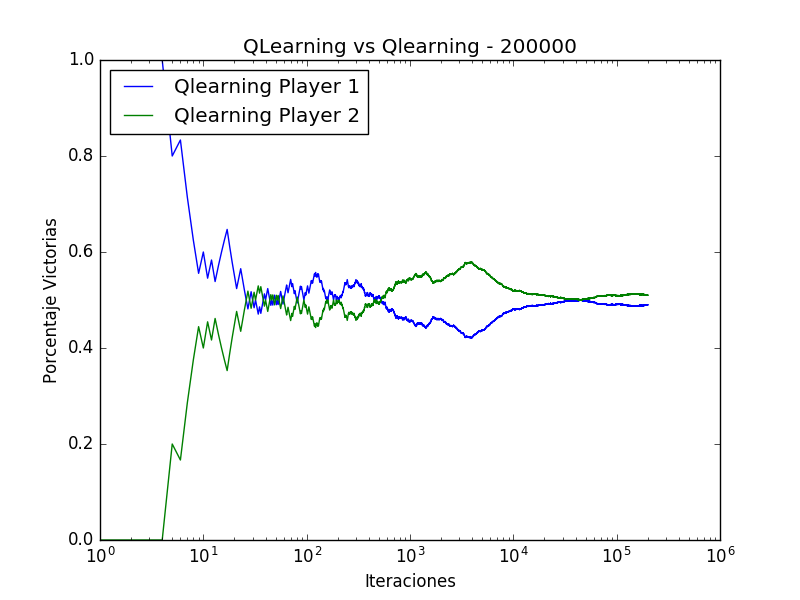
\includegraphics[scale=0.35]{img1/QlearningVsQlearning_200000_6x5_merge_e0p1.png}
        \caption{Qlearning vs Qlearning 200000 juegos - epsilon 1.0}
  \end{minipage}
\end{figure}


Volvimos a jugar contra el jugador entrenado y observamos que ahora si aprendió la estrategia ganadora. Esto explica porque inicialmente cuando jugabamos contra un jugador random los mejores parametros siempre tenían un epsilon bajo, incluso cero. 

Creemos que lo que explica que cuando tenemos dos jugadores Qlearners sin estrategia ganadora lleguen a que nunca se empate tiene que ver con que tener un conjunto grande de estados ganadores, hace que empatar sea dificil y sea mas probable que siempre alguno de los dos gane la partida incluso no conociendo una estrategia ganadora.\\



\subsection{Experimento 4 en linea en tablero de $7\times6$}
Hasta aca jugamos con un tablero de dimensión menor, así que queremos ver si nuestra teoría de que si tenemos un buen conjunto de parametros para el tablero mas chico y el juego tres en línea podemos utilizar el mismo para el juego 4 en linea y obtener buenos resulados.

En esta seccion experimentamos con el tablero original de $7\times6$, y las reglas originales del 4 en linea, obteniendo los siguientes resultados:\\

{\large ACA HAY QUE CORRER DE NUEVO ESTO, NO ME MATEN PERO LOS PARAMETROS FINALES 
CUANDO SE JUEGA CONTRA RANDOM SON: \\
epsilon=0.0001, learning\_rate=0.4, discount=0.9, initialQ=0.0 \\
Y CUANDO SE JUEGA CONTRA OTRO QLEARNING:
epsilon=0.1, learning\_rate=0.4, discount=0.9, initialQ=0.0 \\

HAY QUE CORRER PARA 7x6 4 en linea: \\
iteraciones 200000 para QLEARNING VS RANDOM
iteraciones 200000 para QLEARNING VS QLEARNING
iteraciones 600000 para QLEARNING VS QLEARNING
iteraciones 1000000 para QLEARNING VS QLEARNING

SI LA ULTIMA NO ANDA NO PASA NADA. 

}


\begin{figure}[h]
 \centering
  \begin{minipage}[c]{1\textwidth}
	\centering
	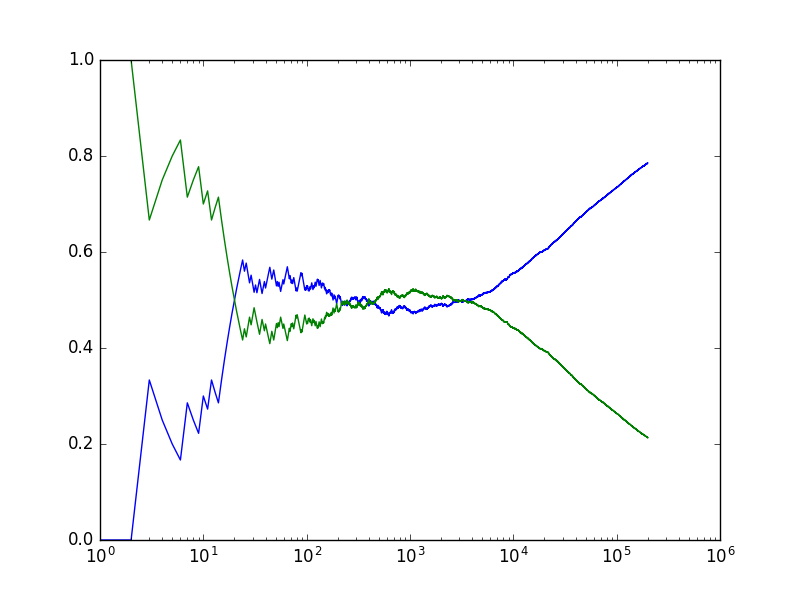
\includegraphics[scale=0.5]{img/QlearningRandomEgreedy2000007x6(4).png}
        \caption{Qlearning vs Random 200000 juegos}
  \end{minipage}
\end{figure}

Lo que podemos observar es bastante razonable, como agrandamos el tablero tenemos muchas mas combinaciones, motivo por el cual, tarda mas tiempo en aprender como ganar.
En este caso ya no encontramos estrategia ganadora para los mismos parametros que en 3 en linea.

Tambien jugamos nosotros contra el Q-learning entrenado y los resultados fueron bastante pobres. 

\begin{figure}[h]
 \centering
 \begin{minipage}{.45\textwidth}
	\centering
	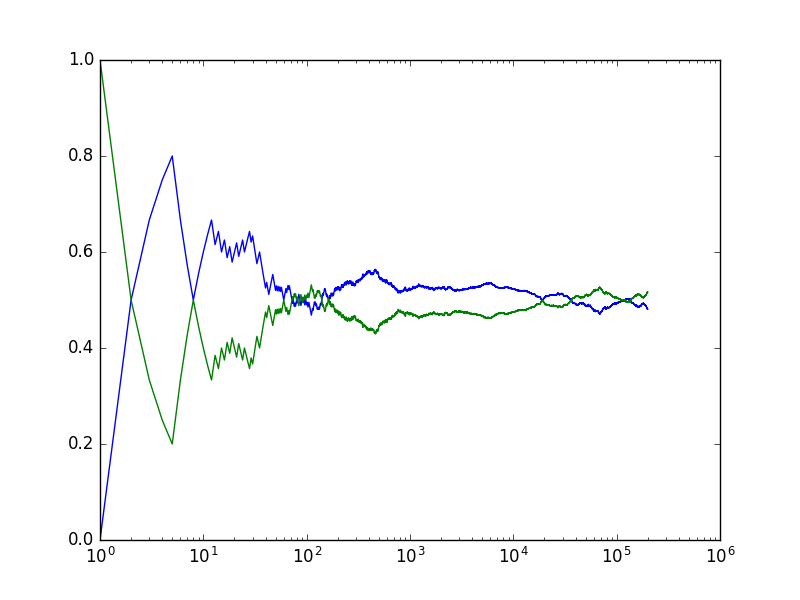
\includegraphics[scale=0.35]{img/QlearningQlearningEgreedy2000007x6(4).png}
       \caption{Qlearning vs Qlearning 200000 juegos}
  \end{minipage}
% \begin{minipage}{.5\textwidth}
%	\centering
%	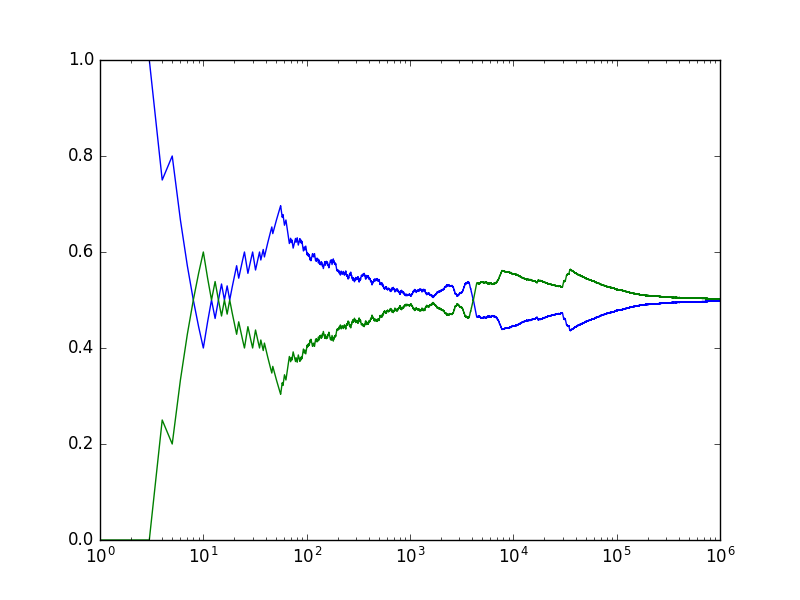
\includegraphics[scale=0.35]{img/QlearningQlearningEgreedy1000000.png}
%        \caption{Qlearning vs Qlearning 1000000 juegos}
%  \end{minipage}
\end{figure}

No pudimos probar Qlearning Vs Qlearning con 9000000 juegos debido al tiempo de computo.



Asi que pensamos en probar otra politica de control: softmax.

Otra vez necesitamos buscar los parametros. En este caso necesitamos definir un tau y una funcion de decremento ademas de textit{learning rate}, \textit{discount}, cantidad de epocas, y los valores de inicializacion de Q. Para estos ultimos exploramos valores que se encontraban alrededor de los encontrados para la estrategia e-greedy.
Empezamos con el tabler de 6x5 y 3 fichas y una vez encontrado los parametros pasamos al tablero real.



{\huge FALTARIA QUE FUNCIONE SOFTMAX Y VER QUE DA. 
LA TEORIA SERIA QUE TIENE QUE SER UN POCO MAS INTELIGENTE PORQUE YA VIMOS QUE LA EXPLORACION LO CAMBIA TODO. 
}\\


{\huge FALTAN CONCLUSIONES
}\\


{\huge SI ALGUIEN SABE COMO HACER PARA QUE RESPETE EL LUGAR DE LOS GRAFICOS GENIAL PORQUE AHORA LOS MEZCLA CON EL TEXTO Y QUEDAN MAL LAS EXPLICACIONES
}\\


%
% \subsection{Experimento 4 en linea en tablero de $7\times6$}
% En el siguiente experimento decidimos entrenar con el juego completo de 4 en linea, en su formato original de un tablero
% de $7\times6$. Para este caso decidimos experimentar con dos politicas de control: \textit{$\epsilon-greedy$} y
% \textit{softmax}. En ambos casos realizamos 500000 iteraciones de juego, y para cada caso entrenamos a nuestro agente
% contra un jugador random y contra otro agente de Qlearning. \\
% Los parametros utilizados tanto para \textit{$\epsilon-greedy$}, como para \textit{softmax} fueron los obtenidos por la
% estrategia de Grid search previamente explicada.
%
% Los resultados obtenidos en cada caso fueron:
%
% \todo{Poner resultados Qlearn vs Qlearn(epsilon greedy)}
%
% \todo{Poner resultados Qlearn vs Qlearn(softmax)}
%
% \todo{Poner resultados Qlearn vs random(epsilon greedy)}
%
% \todo{Poner resultados Qlearn vs random(softmax)}
%
% \subsection{Experimento 3 en linea en tablero de $6\times5$}
